\chapter{Server}
Il passaggio principale che ho dovuto affrontare per l'inizio del progetto è stata l'inizializzazione
di un server che potesse gestire lo scambio di informazioni con l'applicazione ed occuparsi di svolgere tutti i compiti del caso.

Il lavoro del server è facilmente scomponibile in due parti, la gestione dei dati utili per la classificazione 
(che sarà poi affrontata nel capitolo \ref{chapter:classification}) e l'erogazione di dati informativi che vedremo consentire
ad un amministratore l'interazione con il sistema.

Si è scelto di sviluppare il tutto con il linguaggio Python e di inserire per comodità il software in due differenti contenitori Docker, in modo da 
mantenere differenziate queste due parti anche a livello di programmazione.

\subsubsection{Docker}
Docker \cite{docker} è un progetto open-source in grado di effettuare il deploy di applicazioni all'interno di contenitori software che grazie alla
virtualizzazione si trovano ad un livello di astrazione differente dal sistema host. Questa tecnica è molto utile quando si vuole
mantenere separati l'installazione di un applicativo dal sistema ospitante.



\section{RESTful Web API}
\label{section:api}
Come si intuisce in figura \ref{fig:overview}, si è pensato alla creazione di una RESTful Web API.

\subsubsection{Web API}
Una Web API è un'interfaccia composta da un insieme di \textit{endpoints} pubblici che consentono di ottenere informazioni 
o eseguire specifici compiti mediante un processo di richiesta - risposta tra client e server. 

\subsubsection{Architettura REST}
REST (\textit{Representational State Transfer}) è invece un preciso stile architetturale. 

Una RESTful Web API, secondo le specifiche, è dotata di
\begin{itemize}
    \item un \textit{URI} di base (ad esempio, \textit{http://api.example.com/})
    \item metodi HTTP standard (GET, POST, PUT, PATCH e DELETE)
    \item un \textit{media type} che identifica il tipo di dato gestito nel trasferimento 
\end{itemize}

\noindent Gli endpoints realizzati sono utili per ottenere le informazioni durante le fasi preliminari di avvio.
Tutti i componenti interessati a tali informazioni sono in grado di ottenerle con delle richieste.

Si ha accesso ad informazioni sempre aggiornate. Un cambiamento dei valori in fase di amministrazione consente la 
distribuzione delle modifiche senza la necessità di rilasciare un aggiornamento dell'applicazione o riprogrammare il 
\textit{modulo di comunicazione}.


\subsection{Protocollo e formato}
Tutte le richieste e le risposte utilizzano per lo scambio dati il protocollo HTTP, come da specifica REST.
I dati sono trasmessi con il formato JSON.

\subsubsection{HTTP}
HTTP (\textit{HyperText Transfer Protocol}) è un protocollo a livello applicativo per il trasferimento dati. È utilizzato principalmente 
per il trasferimento dati sul web secondo un'architettura client - server.

\subsubsection{JSON}
JSON \cite{json} è un formato standard basato sulla notazione chiave-valore. È famoso per essere facilmente 
leggibile sia da "un umano" che da un calcolatore.



\subsection{Endpoints}
Gli endpoints sono i punti di accesso mediante i quali il software esterno 
è in grado di accedere alle informazioni. La richiesta ad uno specifico URL 
deve restituire una risposta con i dati e le modalità che ci si aspetta.

\begin{listing}[H] 
    \begin{minted}[frame=single,framesep=10pt]{text}
http://IP_ADDRESS:PORT/activities
http://IP_ADDRESS:PORT/positions
http://IP_ADDRESS:PORT/form
    \end{minted}
    \caption{Elenco degli endpoints disponibili}
    \label{listing:endpoint-positions}
\end{listing}

\noindent Gli endpoints che ho previsto sono riservati ad ottenere informazioni su
\begin{itemize}
    \item la lista delle attività classificabili
    \item la lista delle posizioni previste
    \item un modello per la richiesta di informazioni aggiuntive
\end{itemize}


\newpage
\subsubsection{Lista delle attività}
Una richiesta al primo endpoint fornisce la lista di tutte le attività classificabili, nonché di ulteriori informazioni associate ad esse.
\vfill
\begin{listing}[H] 
    \inputminted[frame=single,framesep=10pt]{json}{assets/snippets/server/api/activities.json}
    \caption{Esempio di risposta dell'endpoint delle attività}
    \label{listing:response-activities}
\end{listing}

\newpage
\subsubsection{Lista delle posizioni del dispositivo}
Il secondo endpoint fornisce la lista di tutte le posizioni in cui può essere posizionato il dispositivo durante l'esecuzione 
di una analisi o di un apprendimento.
\vfill
\begin{listing}[H] 
    \inputminted[frame=single,framesep=10pt]{json}{assets/snippets/server/api/positions.json}
    \caption{Esempio di risposta dell'endpoint delle posizioni}
    \label{listing:response-positions}
\end{listing}

\newpage
\subsubsection{Modello per la richiesta di informazioni aggiuntive}
Il terzo endpoint fornisce una struttura per la generazione sull'applicazione di un modulo per la richiesta di dati aggiuntivi. 
Ne discuteremo meglio nel capitolo \ref{chapter:app}.
\vfill
\begin{listing}[H] 
    \inputminted[frame=single,framesep=10pt]{json}{assets/snippets/server/api/form.json}
    \caption{Esempio di risposta dell'endpoint sui dati aggiuntivi}
    \label{listing:response-form}
\end{listing}

\subsection{Implementazione}
L'implementazione del software è stata effettuata con l'utilizzo di Flask. Si occupa di esporre i 
file JSON contenenti le informazioni appena viste nei rispettivi endpoints.

\subsubsection{Flask}
Flask \cite{flask} è uno dei più famosi framework per lo sviluppo di applicazioni web 
con Python. Le sue caratteristiche principali sono leggerezza e semplicità, pur permettendo anche implementazioni 
più avanzate.


\begin{listing}[H] 
    \inputminted[frame=single,framesep=10pt]{python}{assets/snippets/server/api/flask.py}
    \caption{Flask App per una RESTful Web API con 3 endpoints}
\end{listing}



\section{Modulo di Comunicazione}
\label{section:receiver}
Sempre dalla panoramica in figura \ref{fig:overview} è possibile intuire che sul server 
trovano luogo anche il classificatore, i dati che sono stati raccolti e tutti i modelli generati. 

In questa sezione ci occuperemo di ciò che riguarda l'applicativo riservato a gestire la ricezione dei dati e fornire le risposte. 
In particolare la parte del software che si occupa di accettare le connessioni dai client (idealmente l'applicazione realizzata, di cui 
discuteremo nel capitolo \ref{chapter:app}) e di immagazzinare i dati ottenuti.

\subsection{Protocollo e formato}
Avendo la necessità di trasmettere almeno un nuovo messaggio ogni $50ms$ (come vedremo più avanti nel 
paragrafo \ref{paragraph:sampling_rate}), la connessione al \textit{modulo di comunicazione} avviene via socket mediante TCP. 

Trattandosi di un 
protocollo di rete a livello di trasporto ci consente di avere una velocità 
di trasmissione maggiore rispetto a quanto avremmo avuto con HTTP. 

Per comodità si continua ad utilizzare il formato JSON anche in questo frangente per l'organizzazione delle informazioni durante lo scambio dati.


\subsection{Messaggi}
Il \textit{modulo di comunicazione} deve gestire due tipi di richieste, quelle che inviano i dati per effettuarne l'apprendimento e quelle che inviano
i dati in attesa di ricevere il risultato di una classificazione. Malgrado ciò la lettura dei messaggi resta la medesima ed il 
valore per identificare la tipologia di richiesta è disponibile internamente alle informazioni.
\vspace{5mm} %5mm vertical space
\newline
Come mostrato nel codice \ref{listing:example-message-learning}, oltre all'informazione sul tipo di richiesta, un singolo messaggio contiene 
\begin{itemize}
    \item un codice identificante un gruppo di messaggi
    \item un indice indicante la progressione dei dati in quel gruppo
    \item i valori dei 3 assi (x, y, z)
    \item il sensore di movimento che ha generato i valori ottenuti
    \item un valore temporale (\textit{timestamp})
    \item la posizione del telefono selezionata durante l'attività in corso
    \item l'attività che si sta svolgendo (solo nel caso dell'apprendimento)
\end{itemize}
\vfill
\begin{listing}[H] 
    \inputminted[frame=single,framesep=10pt]{json}{assets/snippets/server/receiver/message.json}
    \caption{Esempio di messaggio ricevuto per l'apprendimento}
    \label{listing:example-message-learning}
\end{listing}

\newpage
\subsection{Azioni}
Le azioni da intraprendere per le diverse tipologie di richiesta sono differenti. 

\subsubsection{Messaggi di Apprendimento}
Nel caso della ricezione di dati per l'apprendimento è necessario procedere al salvataggio degli stessi.

\vspace{5mm} %5mm vertical space
I record vengono suddivisi sulla base del relativo sensore. Per ogni sensore si genera un file CSV contenente i record con tutte 
le informazioni rimanenti.

\begin{figure}[H]
    \centering
    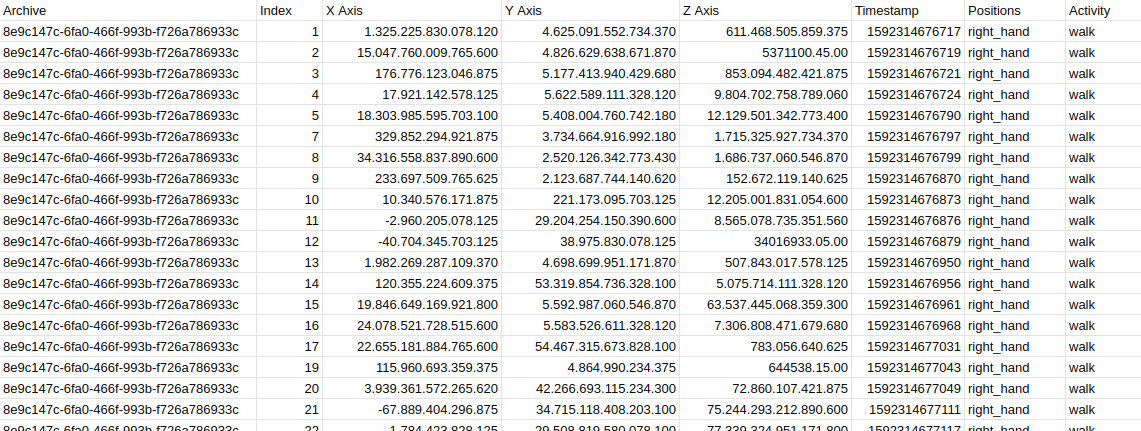
\includegraphics[scale = 0.39]{assets/images/examples/dataset-data-example.png}
    \caption{Esempio del dataset CSV contenente dati accelerometrici}
    \label{fig:example-dataset-csv-accelerometer}
\end{figure}

Ogni volta che la base di dati subisce delle modifiche si avvia il processo di \textit{train} del classificatore, 
trattato nel capitolo \ref{chapter:classification}.


\subsubsection{Messaggi di Analisi}
Nel caso di ricezione di dati per l'analisi non si devono immagazzinare le informazioni ricevute. 
L'obiettivo di questa fase è quello di fornire in risposta al client l'informazione che si aspetta.

Alla ricezione di un numero minimo di record si avvia il processo di classificazione, trattato sempre nel capitolo \ref{chapter:classification}.
L'ipotesi ottenuta dal classificatore sarà inviata come risposta.
\vfill
\begin{listing}[H] 
    \inputminted[frame=single,framesep=10pt]{json}{assets/snippets/server/receiver/prediction.json}
    \caption{Esempio del messaggio di risposta con l'ipotesi formulata}
    \label{listing:example-message-prediction}
\end{listing}